\documentclass[10pt,a4paper]{article}
\usepackage[utf8]{inputenc}

% \usepackage{ngerman}  % german documents
\usepackage{graphicx}  % import graphics einbinden
\usepackage{listings}  % support source code listing
\usepackage{amsmath}  % math stuff
\usepackage{amssymb} % 
\usepackage{a4wide} % wide pages
\usepackage{fancyhdr} % nice headers
\usepackage{tikz} %graphs
\usetikzlibrary{arrows}
\lstset{basicstyle=\footnotesize,language=Python,numbers=left, numberstyle=\tiny, stepnumber=5,firstnumber=0, numbersep=5pt} % set up listings
\pagestyle{fancy}             % header
\setlength{\parindent}{0pt}   % no indentation

\usepackage[pdfpagemode=None, colorlinks=true,  % url coloring
           linkcolor=blue, urlcolor=blue, citecolor=blue, plainpages=false, 
           pdfpagelabels,unicode]{hyperref}
           
% change enums style: first level (a), (b), (c)           
\renewcommand{\labelenumi}{(\alph{enumi})}
\renewcommand{\labelenumii}{(\arabic{enumii})}

%lecture name
\newcommand{\lecture}{
	Bioinformatics III
}           

%assignment iteration
\newcommand{\assignment}{
	Seventh Assignment
}

%set up names, matricle number, and email
\newcommand{\authors}{
  \begin{tabular}{rl}
    \href{mailto:s9alfloh@stud.uni-saarland.de}{Alexander Flohr} & (2549738)\\
    \href{mailto:s9ankupi@stud.uni-saarland.de}{Andrea Kupitz} & (2550260)
  \end{tabular}
}

% use to start a new exercise
\newcommand{\exercise}[1]
{
  \stepcounter{subsection}
  \subsection*{Exercise \thesubsection: #1}

}

\begin{document}
\title{\Large \lecture \\ \textbf{\normalsize \assignment}}
\author{\authors}

\setlength \headheight{25pt}
\fancyhead[R]{\begin{tabular}{r}\lecture \\ \assignment \end{tabular}}
\fancyhead[L]{\authors}


\setcounter{section}{7} % modify for later sheets, i.e. 2, 3, ...
%\section{Introduction to Python and some Network Properties} % optional, note that section invocation sets the section counter + 1, so adapt the setcounter command
\maketitle

\exercise{Missing Data Imputation}
\begin{enumerate}
\item \lstinputlisting[tabsize=4, label=ex1-a1,caption={Listing of source code}] {imput.R}
Listing \ref{ex1-a1} shows the source code of our imputation of data. Figure \ref{fig-1} shows the imputed data.\\
\begin{figure}
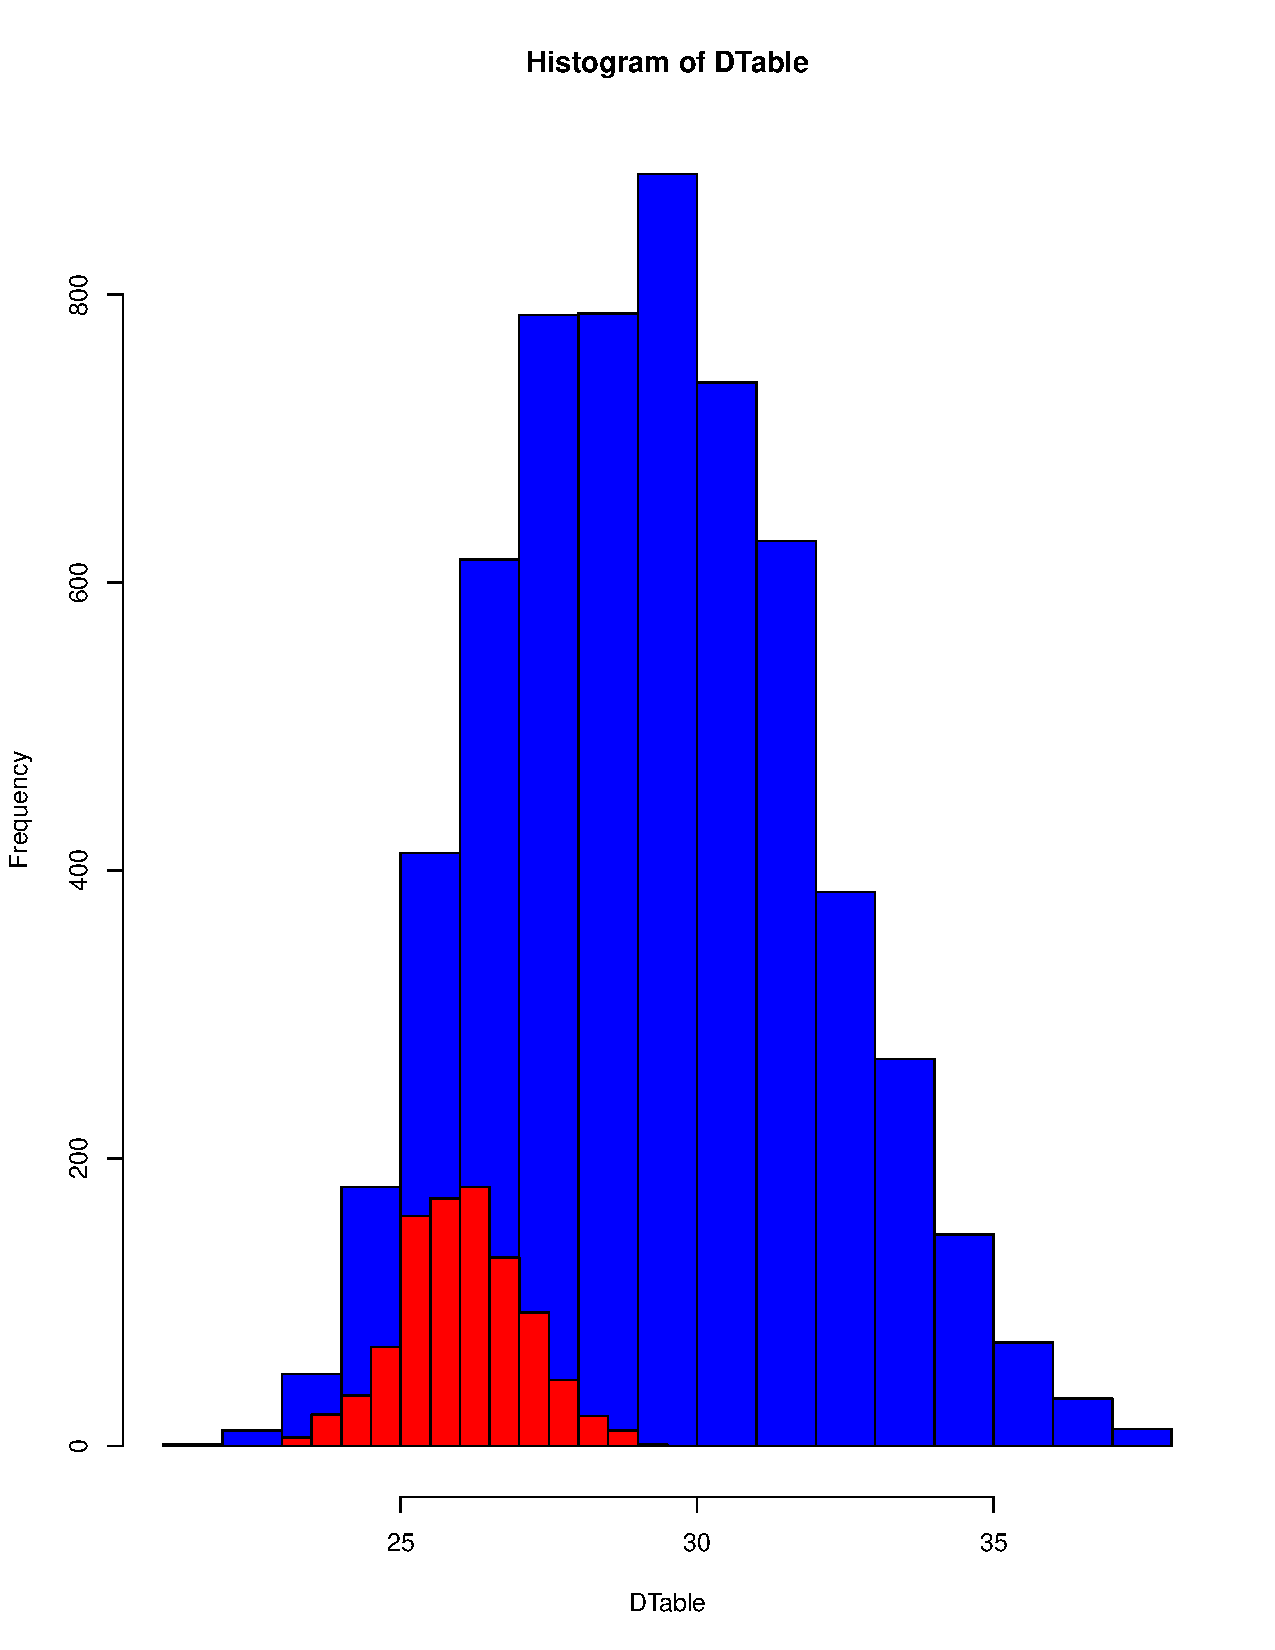
\includegraphics[scale=0.3]{Hist0.pdf}
\caption{Distribution of the sample with the imputed data}
\label{fig-1}
\end{figure}
\item The greater the standard deviation gets, the wider gets the histogram of the imputated data. Moreover for greater standard deviations the values tend to lay more far away from each other and thus the single bars of the histogram are lower.\\
The closer the new mean moves to the original mean, the more moves the distribution of the imputated data to the center of the original data.\\
Figures \ref{fig-2}, \ref{fig-3}, \ref{fig-4} show the imputated data with increasing mean.\\
Figures \ref{fig-5}, \ref{fig-6}, \ref{fig-7} show the imputated data with increasing standard deviation.\\
\begin{figure}
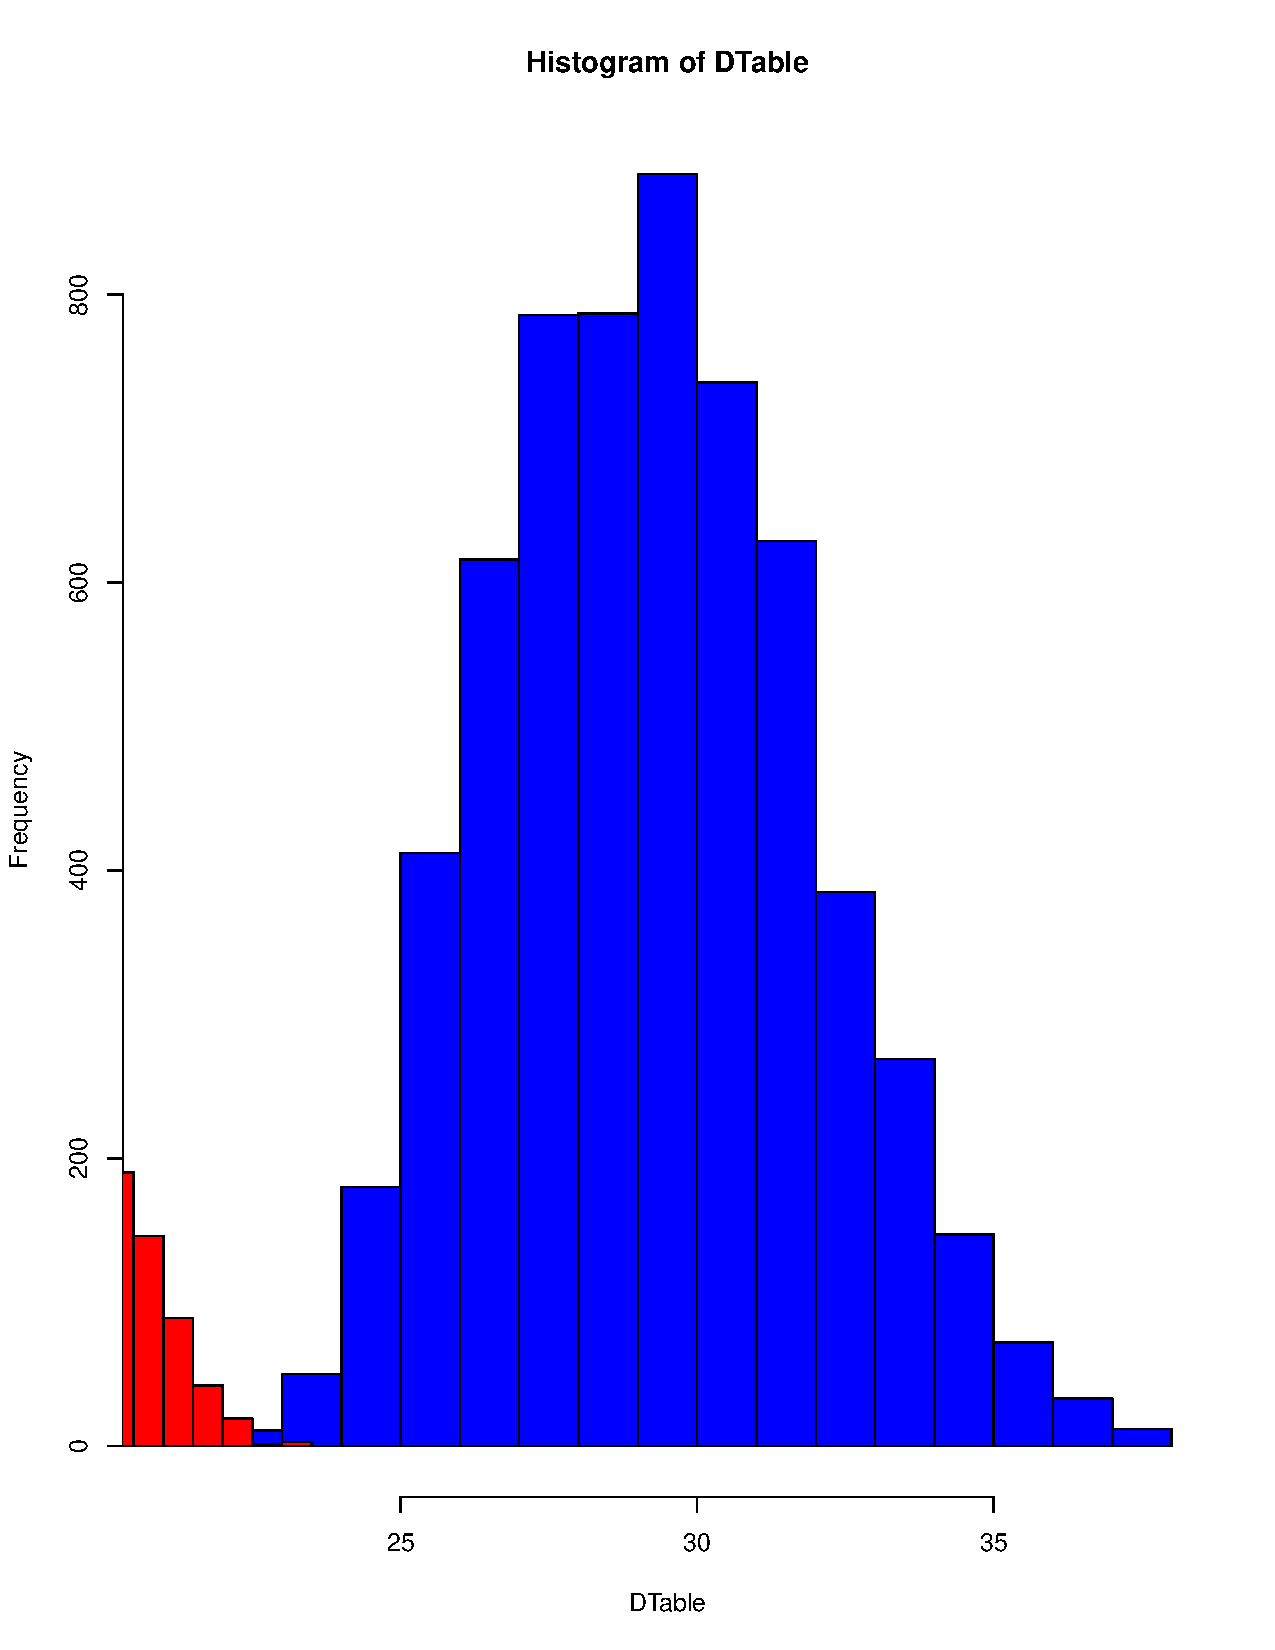
\includegraphics[scale=0.3]{Hist1.pdf}
\caption{Distribution of the sample with the imputed data}
\label{fig-2}
\end{figure}
\begin{figure}
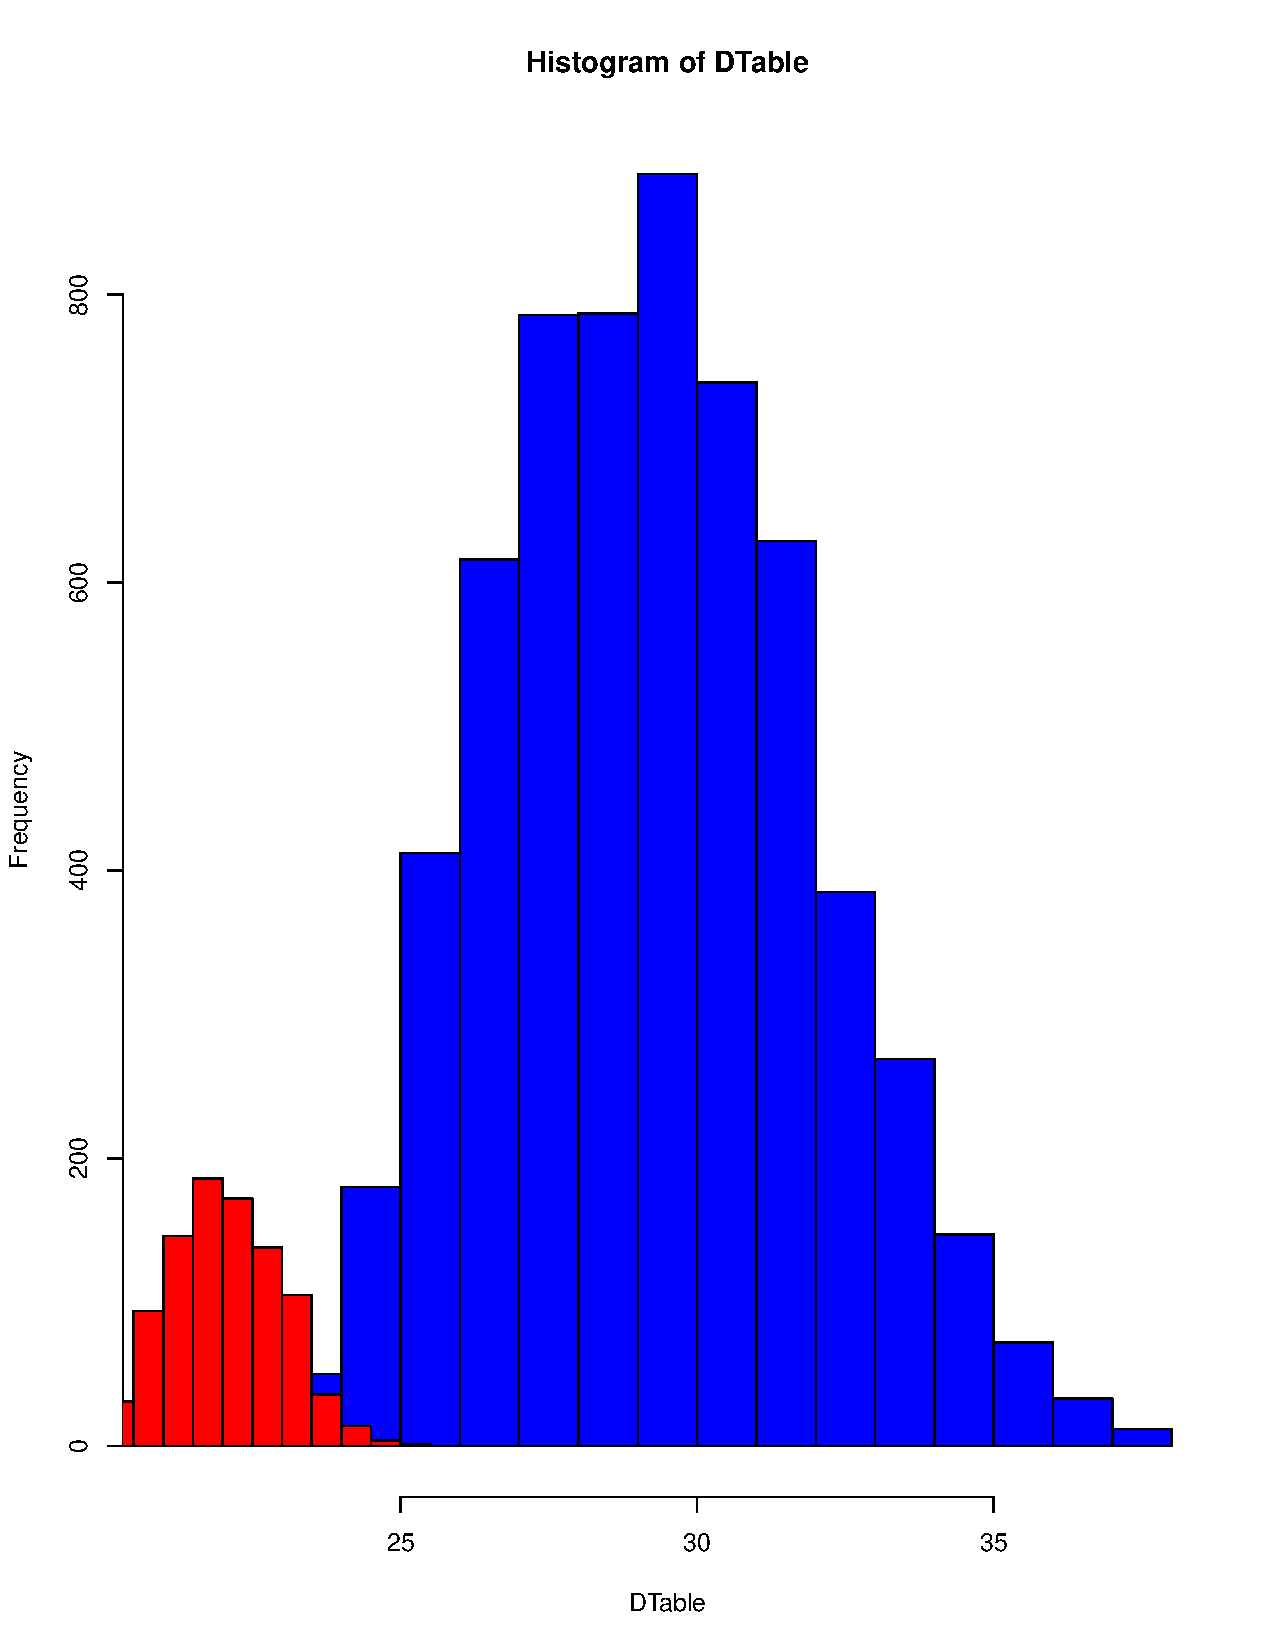
\includegraphics[scale=0.3]{Hist2.pdf}
\caption{Distribution of the sample with the imputed data}
\label{fig-3}
\end{figure}
\begin{figure}
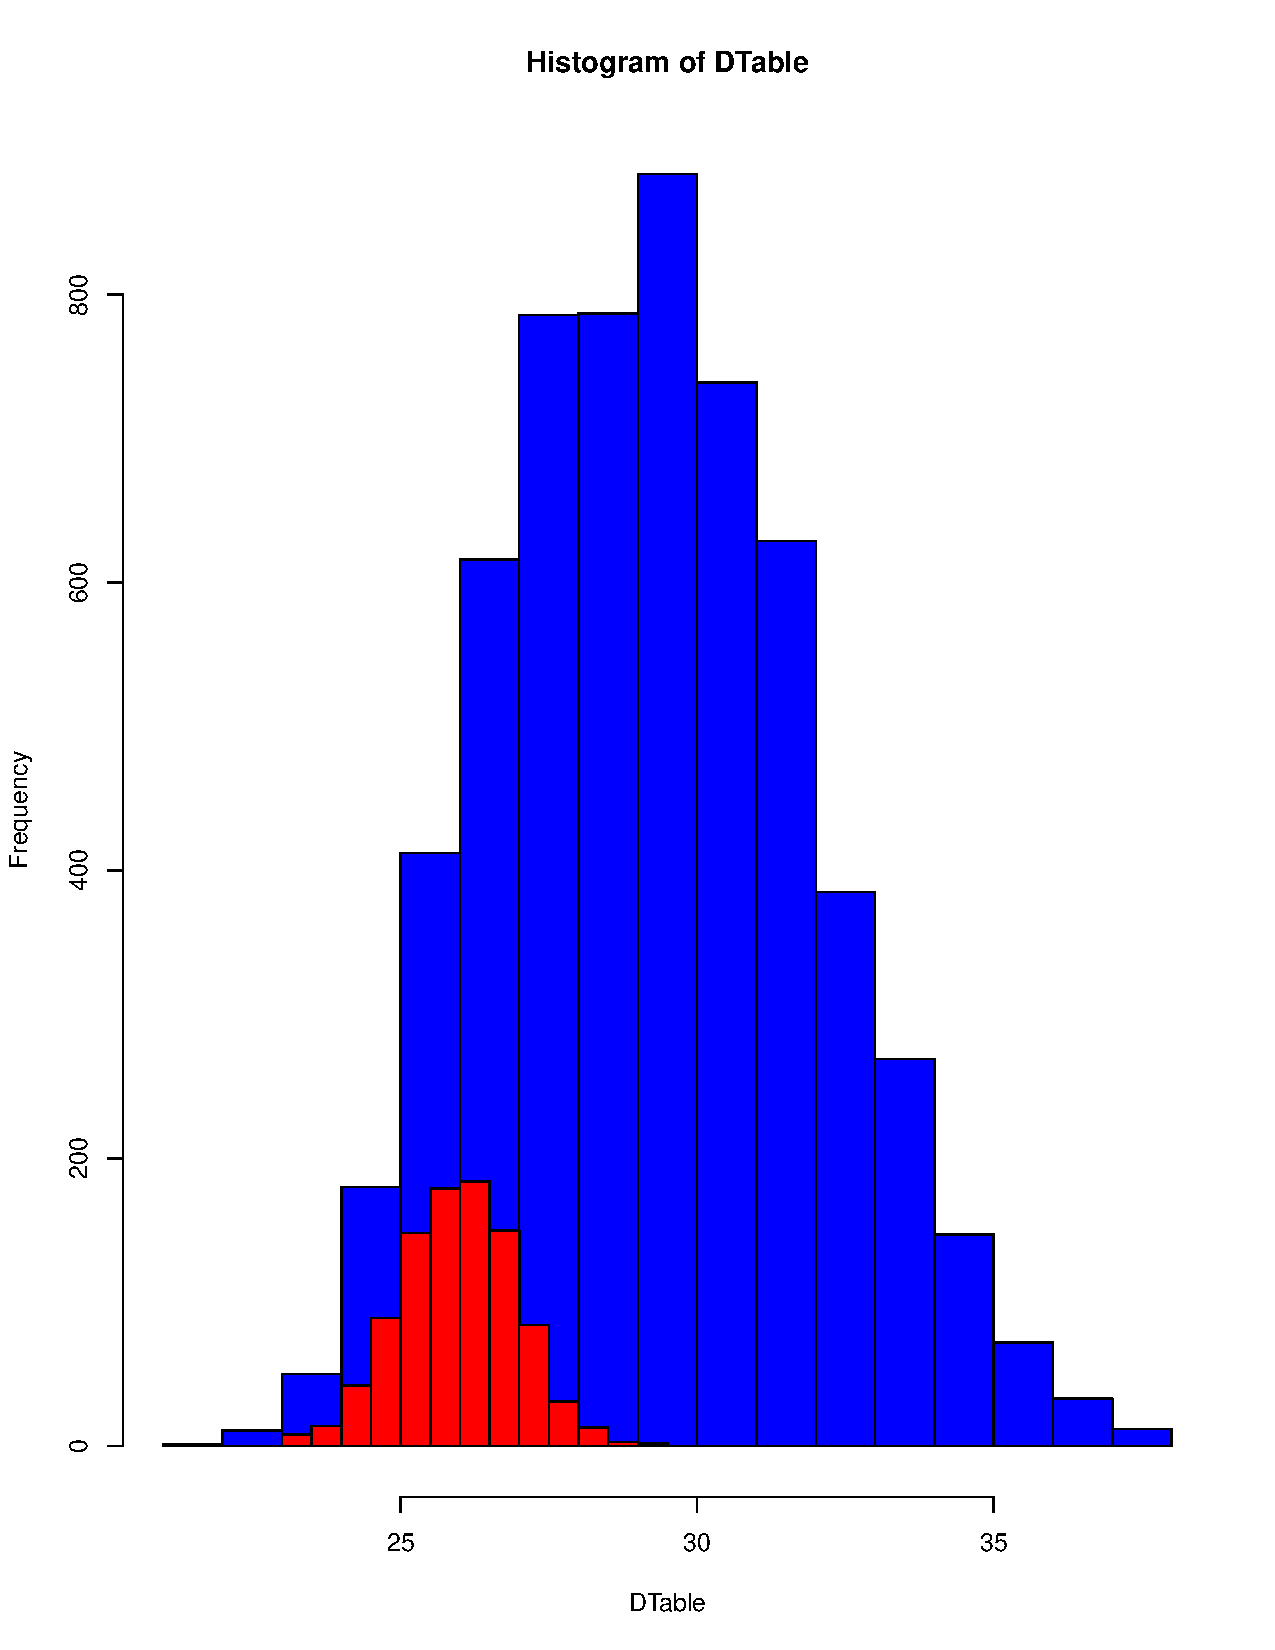
\includegraphics[scale=0.3]{Hist3.pdf}
\caption{Distribution of the sample with the imputed data}
\label{fig-4}
\end{figure}
\begin{figure}
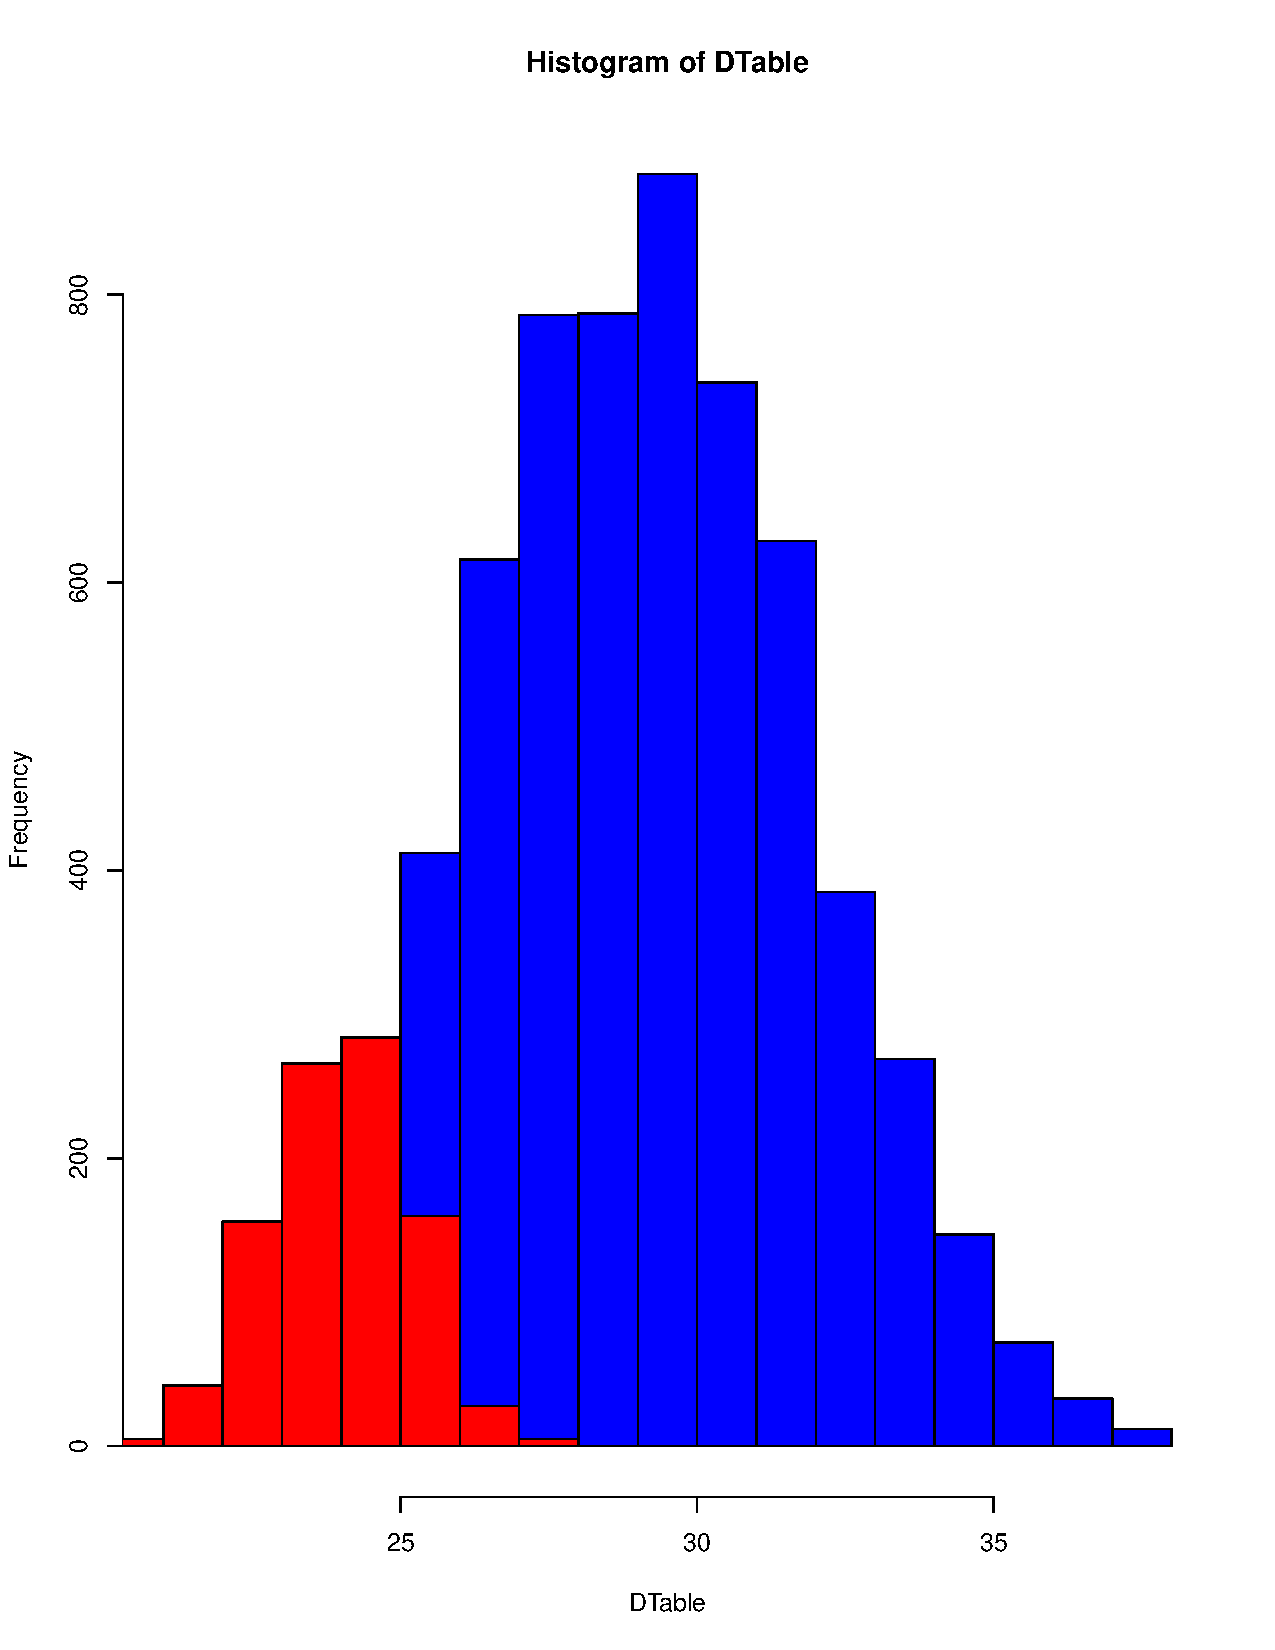
\includegraphics[scale=0.3]{Hist4.pdf}
\caption{Distribution of the sample with the imputed data}
\label{fig-5}
\end{figure}
\begin{figure}
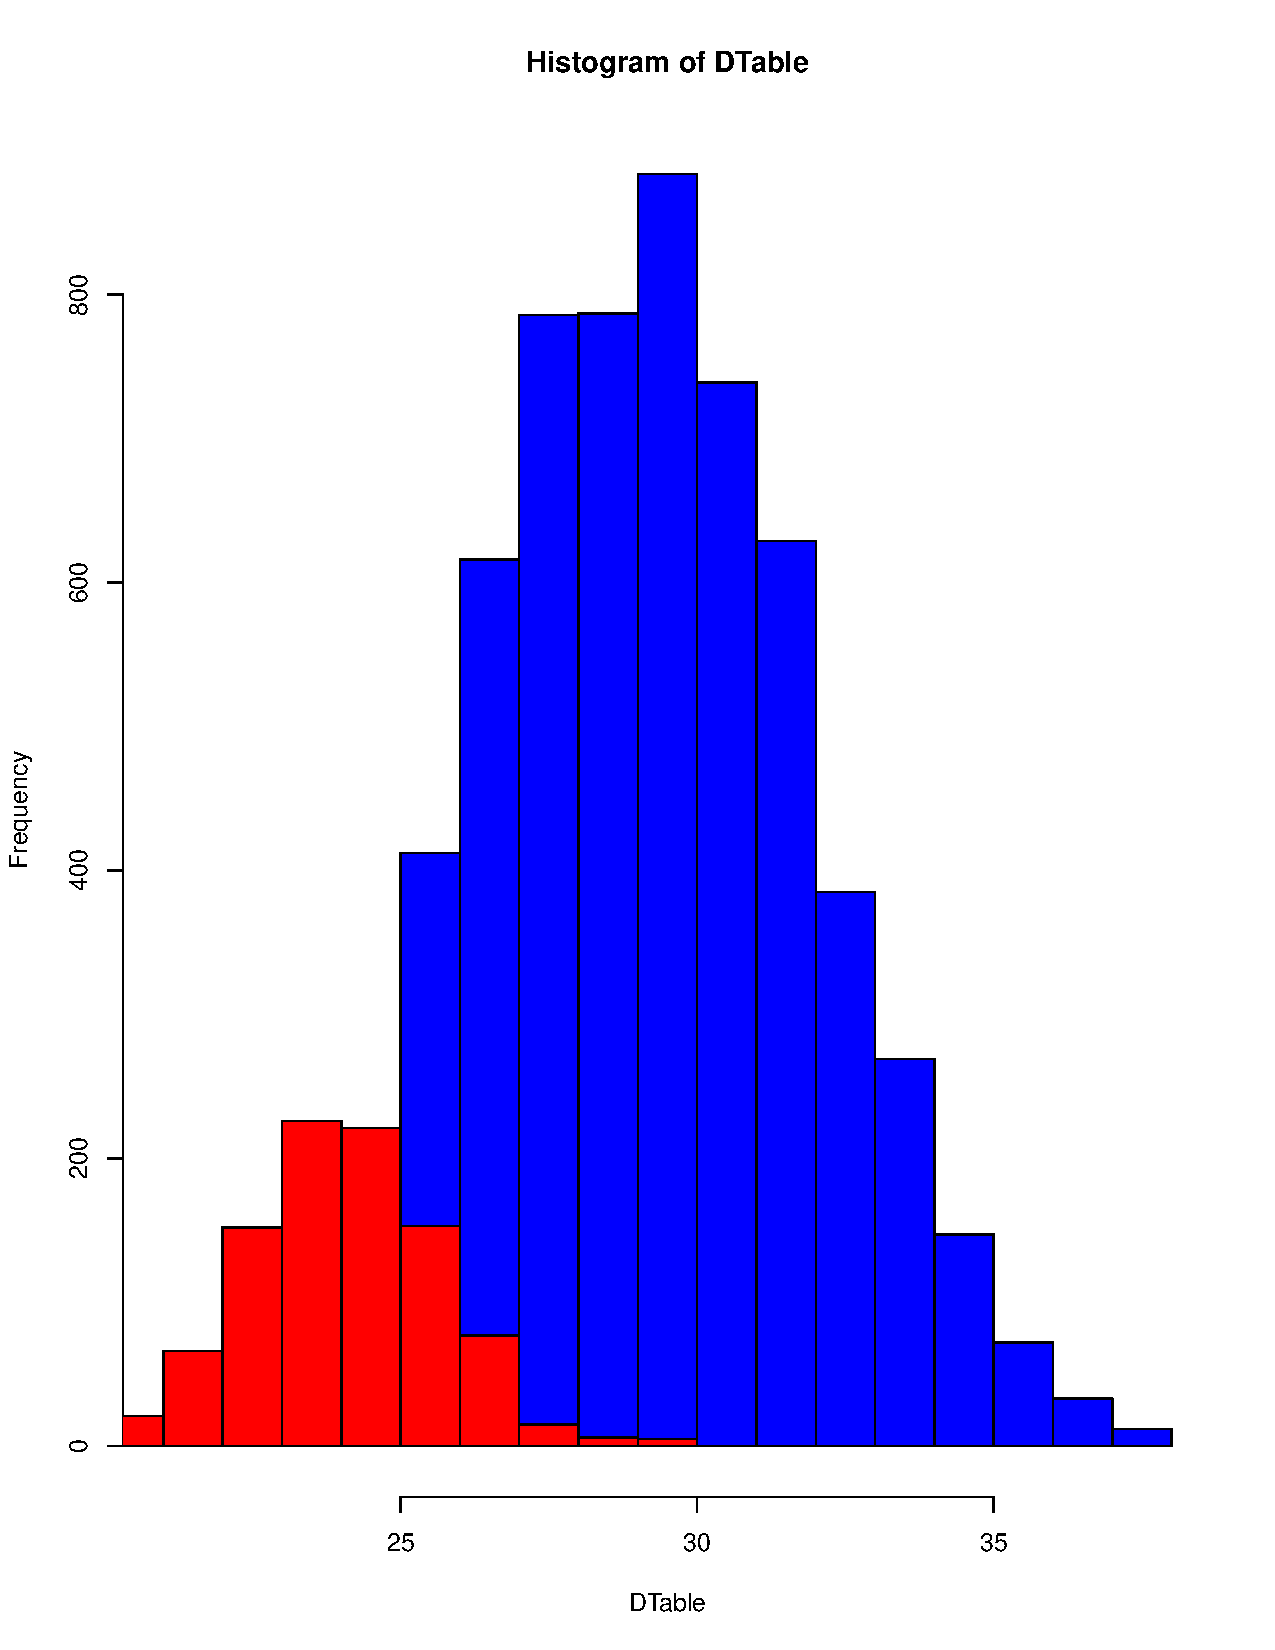
\includegraphics[scale=0.3]{Hist5.pdf}
\caption{Distribution of the sample with the imputed data}
\label{fig-6}
\end{figure}
\begin{figure}
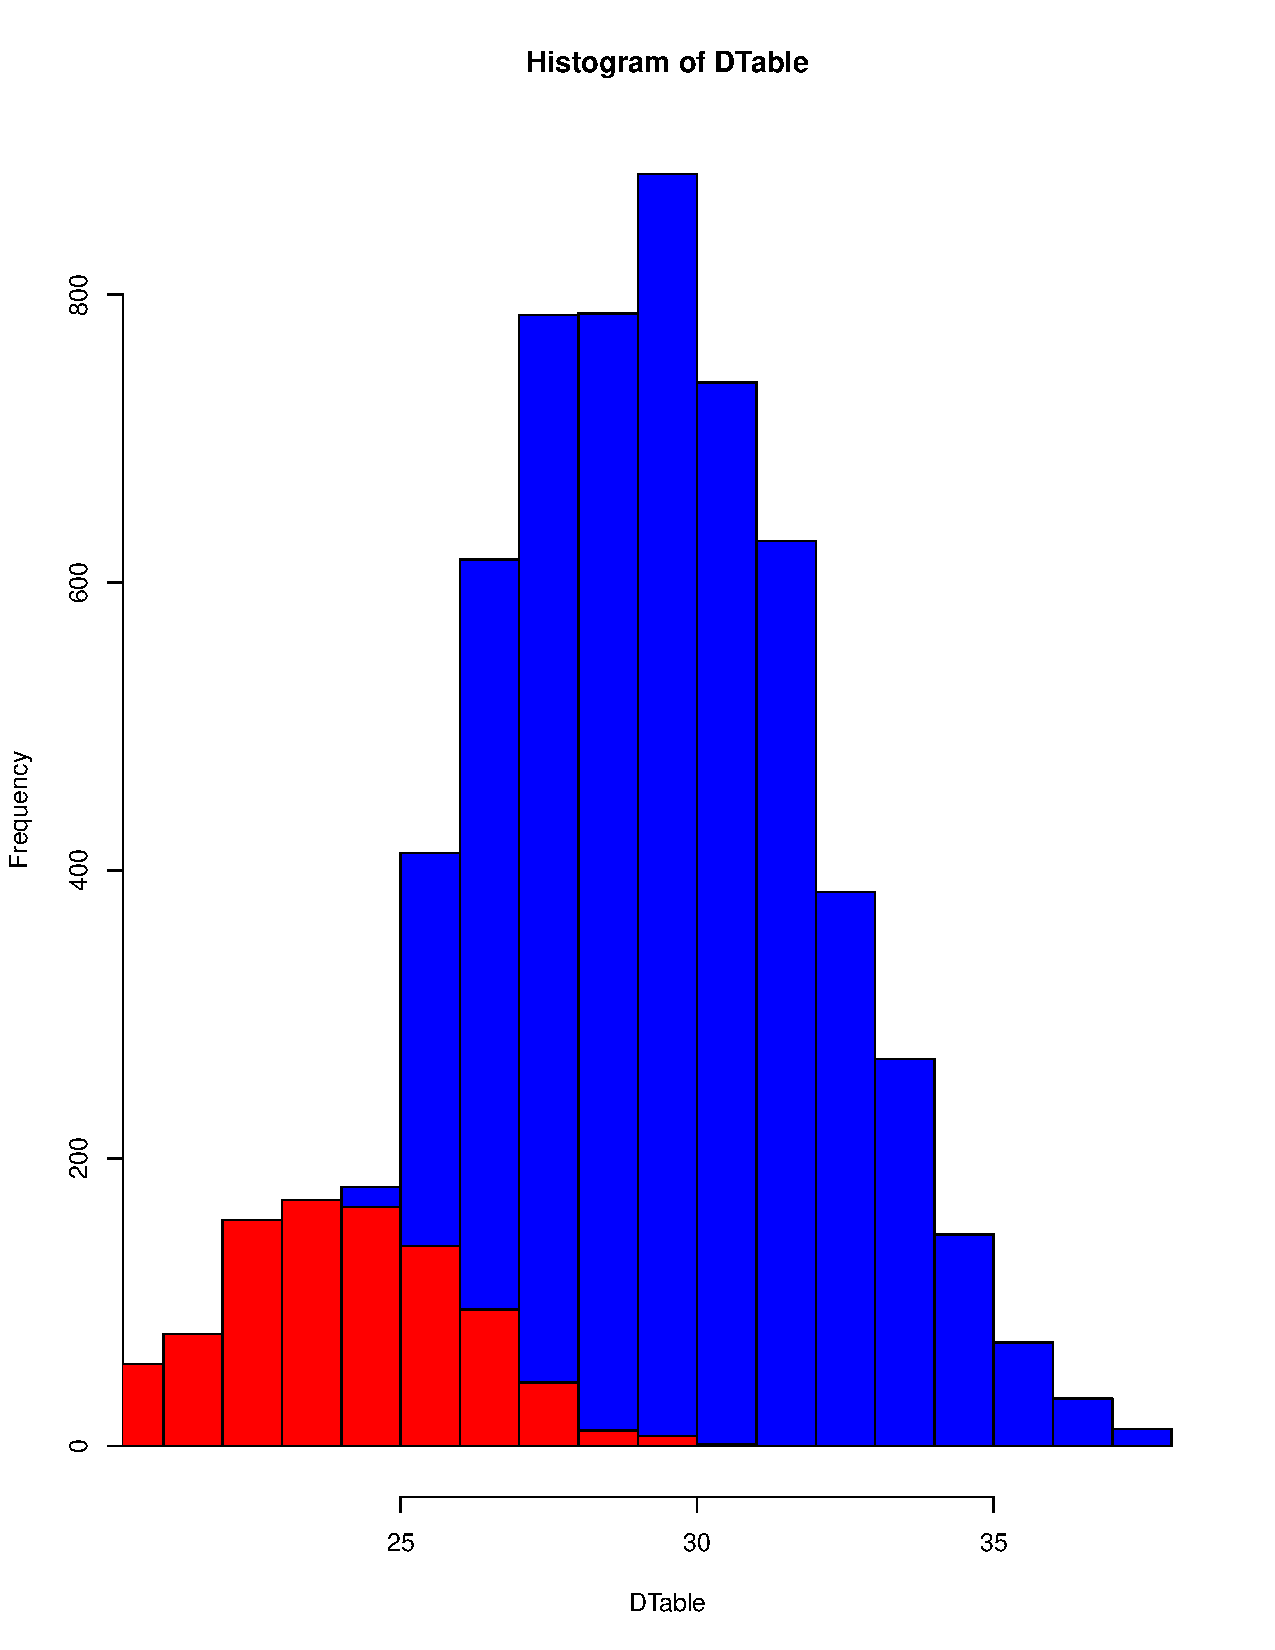
\includegraphics[scale=0.3]{Hist6.pdf}
\caption{Distribution of the sample with the imputed data}
\label{fig-7}
\end{figure}
\end{enumerate}

\newpage
\exercise{DREAM challenge}
Listing \ref{ex2} shows the R implementation of the noise modle. We used 1000 iterations to refine the modle.
\lstinputlisting[tabsize=4, label=ex2,caption={Listing of source code}] {ex_7_2.R}

Output:\\
\texttt{G7	G10	0\\
G4	G6	0.00282553\\
G2	G6	0.01111409\\
G3	G6	0.01395305\\
G6	G5	0.02255766\\
G10	G5	0.02255766\\
G5	G6	0.02788807\\
G6	G7	0.04557906\\
G8	G7	0.04557906\\
}
Less iterations could increase the number of predicted links bout might be less precise.

\end{document}